% This LaTeX was auto-generated from MATLAB code.
% To make changes, update the MATLAB code and export to LaTeX again.

\documentclass{article}

\usepackage[utf8]{inputenc}
\usepackage[T1]{fontenc}
\usepackage{lmodern}
\usepackage{graphicx}
\usepackage{color}
\usepackage{hyperref}
\usepackage{amsmath}
\usepackage{amsfonts}
\usepackage{epstopdf}
\usepackage[table]{xcolor}
\usepackage{matlab}

\sloppy
\epstopdfsetup{outdir=./}
\graphicspath{ {./le_4_3_4_images/} }

\begin{document}

\matlabtitle{Algebra}

\begin{matlabcode}
clear; syms s w
A = [0 -1 0;1 0 1;0 0 0];
C = [1 0 0];
K = sym('K',[3 1]);
% s*eye(3) - A + K*C
e1 = collect(det(s*eye(3) - A + K*C),s);
e2 = collect((s + 0.1)*(s + 0.1)*(s + 10),s);
c1 = coeffs(e1,s); c1(end) = []; 
c2 = coeffs(e2,s); c2(end) = [];
eqns = c1 == c2;
Sol = solve(eqns,K);
%%% reduced order
% Ar = A(2:3,1:2);
Ar = [0 0; 1 0];
% cr = A(1,1:2);
cr = [0 -1];
L = sym('L',[2 1]);
% s*eye(2) - Ar + L*cr;
er1 = collect(det(s*eye(2) - Ar + L*cr),s);
er2 = collect((s + 0.1)*(s + 0.1),s);
cr1 = coeffs(er1,s); cr1(end) = []; 
cr2 = coeffs(er2,s); cr2(end) = [];
eqnrs = cr1 == cr2;
Solr = solve(eqnrs,L);
\end{matlabcode}


\matlabheading{simulation (true system)u = 1 ; \% input \% state space representation [x; xdot; y; ydot]}

\begin{matlabcode}
clear;
u = 10;
A = [0 -1 0; 1 0 1; 0 0 0];
B = [0; 0; 1]; C = [1 0 0];
int_nav = @(t,x) A*x + B*u;

% simulation
y0 = [0; 0; 0]; % initial states
tspan = [0 80]; % [s]
[t, y] = ode45(@(t,y) int_nav(t,y),tspan,y0);
\end{matlabcode}


\matlabheading{Observer simulation}

\begin{matlabcode}
% state observer 
K = [10.2; -1.01; -0.1];
mesh = @(x) interp1(t,y(:,1),x,'spline');
obs_int_nav = @(t,x) A*x + B*u + K*(mesh(t) - C*x);

% simulation 
y0 = [0; 2; 10]; % initial states
[to, yo] = ode45(@(t,y) obs_int_nav(t,y),tspan,y0); 

% error
for ii = 1:width(y)
    yq = interp1(t,y(:,ii),to);
    eq(:,ii) = yq - yo(:,ii);
end
\end{matlabcode}


\matlabheading{Second-order observer}

\begin{matlabcode}
% A-matrix partition
Ar = [0 0; 1 0];
cr = [0 -1];
br = [0; 1];
ann = 0;
% B_matrix
gr = [1; 0];
gn = 0;
% observer gain
L = [-0.01; -0.2];
% state observer
red_obs_int_nav = @(t,z) (Ar - L*cr)*z + (br -L*ann + Ar*L - L*cr*L)*mesh(t) + (gr - L*gn)*u;

% simulation
y0 = [10; 2]; % initial states
[tr, zo] = ode45(@(t,y) red_obs_int_nav(t,y),tspan,y0); 

% states
for ii = 1:length(tr)
    xr(ii,:) = zo(ii,:) + (L*mesh(tr(ii)))';
end

% error
yq = interp1(t,y(:,3),tr);
eq2(:,1) = yq - xr(:,1);
yq = interp1(t,y(:,2),tr);
eq2(:,2) = yq - xr(:,2);
\end{matlabcode}


\matlabheading{plots}

\begin{matlabcode}
figure(1); clf; tiledlayout(3,2)
ax(1) = nexttile; plot(t,y(:,1),to,yo(:,1),'LineWidth',2); box off
ylabel('$v$ [m/s]','Interpreter',"latex"); xlabel('$t$ [s]','Interpreter',"latex");
ax(2) = nexttile; plot(to,eq(:,1),'LineWidth',2); box off
ylabel('$\tilde v$ [m/s]','Interpreter',"latex"); xlabel('$t$ [s]','Interpreter',"latex");
ax(3) = nexttile; plot(t,y(:,2),to,yo(:,2),'LineWidth',2); box off
ylabel('$\varphi$ [m]','Interpreter',"latex"); xlabel('$t$ [s]','Interpreter',"latex");
ax(4) = nexttile; plot(to,eq(:,2),'LineWidth',2); box off
ylabel('$\tilde{\varphi}$ [m]','Interpreter',"latex"); xlabel('$t$ [s]','Interpreter',"latex");
ax(5) = nexttile; plot(t,y(:,3),to,yo(:,3),'LineWidth',2); box off
ylabel('$\varepsilon$ [m]','Interpreter',"latex"); xlabel('$t$ [s]','Interpreter',"latex");
ax(6) = nexttile; plot(to,eq(:,3),'LineWidth',2); box off
ylabel('$\tilde{\varepsilon}$ [m]','Interpreter',"latex"); xlabel('$t$ [s]','Interpreter',"latex");
linkaxes(ax,'x'); clear ax;
% saving plots
textwidth = 13.6;
golden_ratio = (1 + sqrt(5)) / 2 ;
textheight = textwidth / golden_ratio * 1.5;
figsize = [textwidth, textheight];

% Get latex font in ticks
h = findall(gcf,'Type','axes'); % An array if you have subplots
set(h, 'TickLabelInterpreter', 'latex')
\end{matlabcode}
\begin{center}
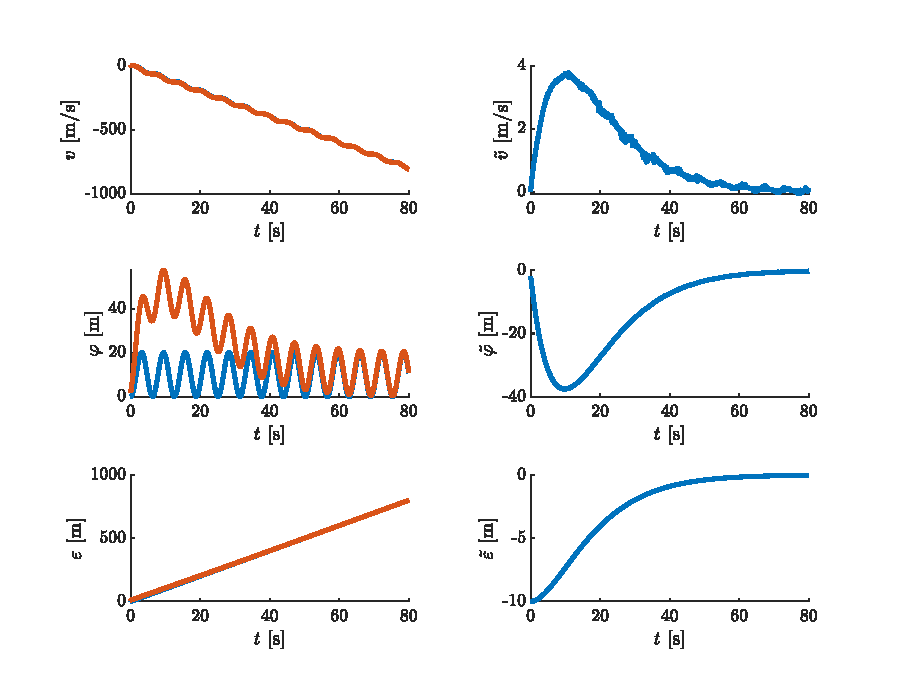
\includegraphics[width=\maxwidth{56.196688409433015em}]{figure_0.eps}
\end{center}
\begin{matlabcode}

% Set size and no crop
set(gcf, 'PaperUnits', 'centimeters', 'PaperSize', figsize);
set(gcf, 'PaperUnits', 'normalized', 'PaperPosition', [0, 0, 1, 1]);

% save results 
% print -dpdf ../doc/figures/le4_3_7a.pdf
\end{matlabcode}


\matlabheading{plots 2}

\begin{matlabcode}
figure(2); clf; tiledlayout(2,2)
ax(1) = nexttile; plot(t,y(:,2),tr,xr(:,2),'LineWidth',2); box off
ylabel('$\varphi$ [m]','Interpreter',"latex"); xlabel('$t$ [s]','Interpreter',"latex");
ax(2) = nexttile; plot(tr,eq2(:,2),'LineWidth',2); box off
ylabel('$\tilde{\varphi}$ [m]','Interpreter',"latex"); xlabel('$t$ [s]','Interpreter',"latex");
ax(3) = nexttile; plot(t,y(:,3),tr,xr(:,1),'LineWidth',2); box off
ylabel('$\varepsilon$ [m]','Interpreter',"latex"); xlabel('$t$ [s]','Interpreter',"latex");
ax(4) = nexttile; plot(tr,eq2(:,1),'LineWidth',2); box off
ylabel('$\tilde{\varepsilon}$ [m]','Interpreter',"latex"); xlabel('$t$ [s]','Interpreter',"latex");
linkaxes(ax,'x'); clear ax;
% saving plots
textwidth = 13.6;
golden_ratio = (1 + sqrt(5)) / 2 ;
textheight = textwidth / golden_ratio;
figsize = [textwidth, textheight];

% Get latex font in ticks
h = findall(gcf,'Type','axes'); % An array if you have subplots
set(h, 'TickLabelInterpreter', 'latex')

% Set size and no crop
set(gcf, 'PaperUnits', 'centimeters', 'PaperSize', figsize);
set(gcf, 'PaperUnits', 'normalized', 'PaperPosition', [0, 0, 1, 1]);

% save results 
% print -dpdf ../doc/figures/le4_3_7b.pdf
\end{matlabcode}

\end{document}
